\documentclass{report}
\usepackage[utf8]{inputenc}
\usepackage{graphicx}
\begin{document}

\chapter{6. Availability}
\section{Availability}

Some systems we need to	be there whenever they need to be used.	These are usually called high availability systems.	
There can be different reasons for high availability:	
\begin{itemize}
\item{999 telephone system}
\item{Interplanetary spacecraft systems}
\item{Electricity supply grid}
\item{Large Computer System Power Supply}
\end{itemize}

From Hardware, there are two key measures:
\begin{itemize}
\item{MTBF: Mean Time Between Failures}
\item{MTTR: Mean Time To Repair}
\end{itemize}
Availability is the probability of the system working, when you ask it to work.\newline

$\textit{availability = }\frac{MTBF}{MTBF+MTTR}$\newline

To maximise the probability, either make the time between failures larger, or a quicker repair time.
\newline
\section{Faults, errors, and failures}
A fault is something in the system (e.g. a broken wire, failed component, wrong bit of code, …)	that can cause the system to move into an error	state when the fault is activated, an error may then eventually cause an externally observable deviation from the intended operation and this is called a failure.\newline

Most high availability systems try to tolerate or mask faults by detecting erroneous conditions before they move into failure	conditions. 

\section{Faults, errors, and failures - Example}
A fault in a sorting routine means that under some circumstances it fails to sort an array.\newline

Under these conditions, the system might be assuming an array is sorted but it isn’t.  In this state there is an error in the system because things are not as they should be.\newline

If the system uses binary search to look for things in the array, sometimes an item will be in the array but will not be found – this might cause a visible failure  of the system.

\section{Generic Scenario}

\begin{itemize}
\item{\textbf{Source}: Internal or external sources important to differentiate because different measures are possible.}
\item{\textbf{Stimulus}: Fault causes errors: omission (no result), crash (repeated omissions), timing (late, early), response (incorrect value).}
\item{\textbf{Artifact}: Specifies what has to be available: process, channel, store, …}
\item{\textbf{Environment}: what the mode of operation is: normal, degraded, startup, shutdown, …}
\item{\textbf{Response}:  how to respond to the stimulus }
\item{\textbf{Response measure}: this will be some measure related to the availability or the “liveness” of the artifact}
\end{itemize}

\section{Concrete Scenario}

In mission critical systems there is typically a schedule that activates a sequence of tasks in turn.  These take longer or shorter times to complete and the whole set is carried out cyclically. What happens if there is a bug in a task and it never completes?

\begin{itemize}
\item{Cycles through each of the tasks.}
\item{Passes control to one of the tasks}
\item{Waits for control to pass back.}
\item{If one of the task fails, the architecture fails the scenario.}
\end{itemize}

\pagebreak
\section{Availability Tactics}

If our architecture fails the scenario, because we can't detect the error arising from the fault in one of our tasks, we look at the tactics:
\begin{center}
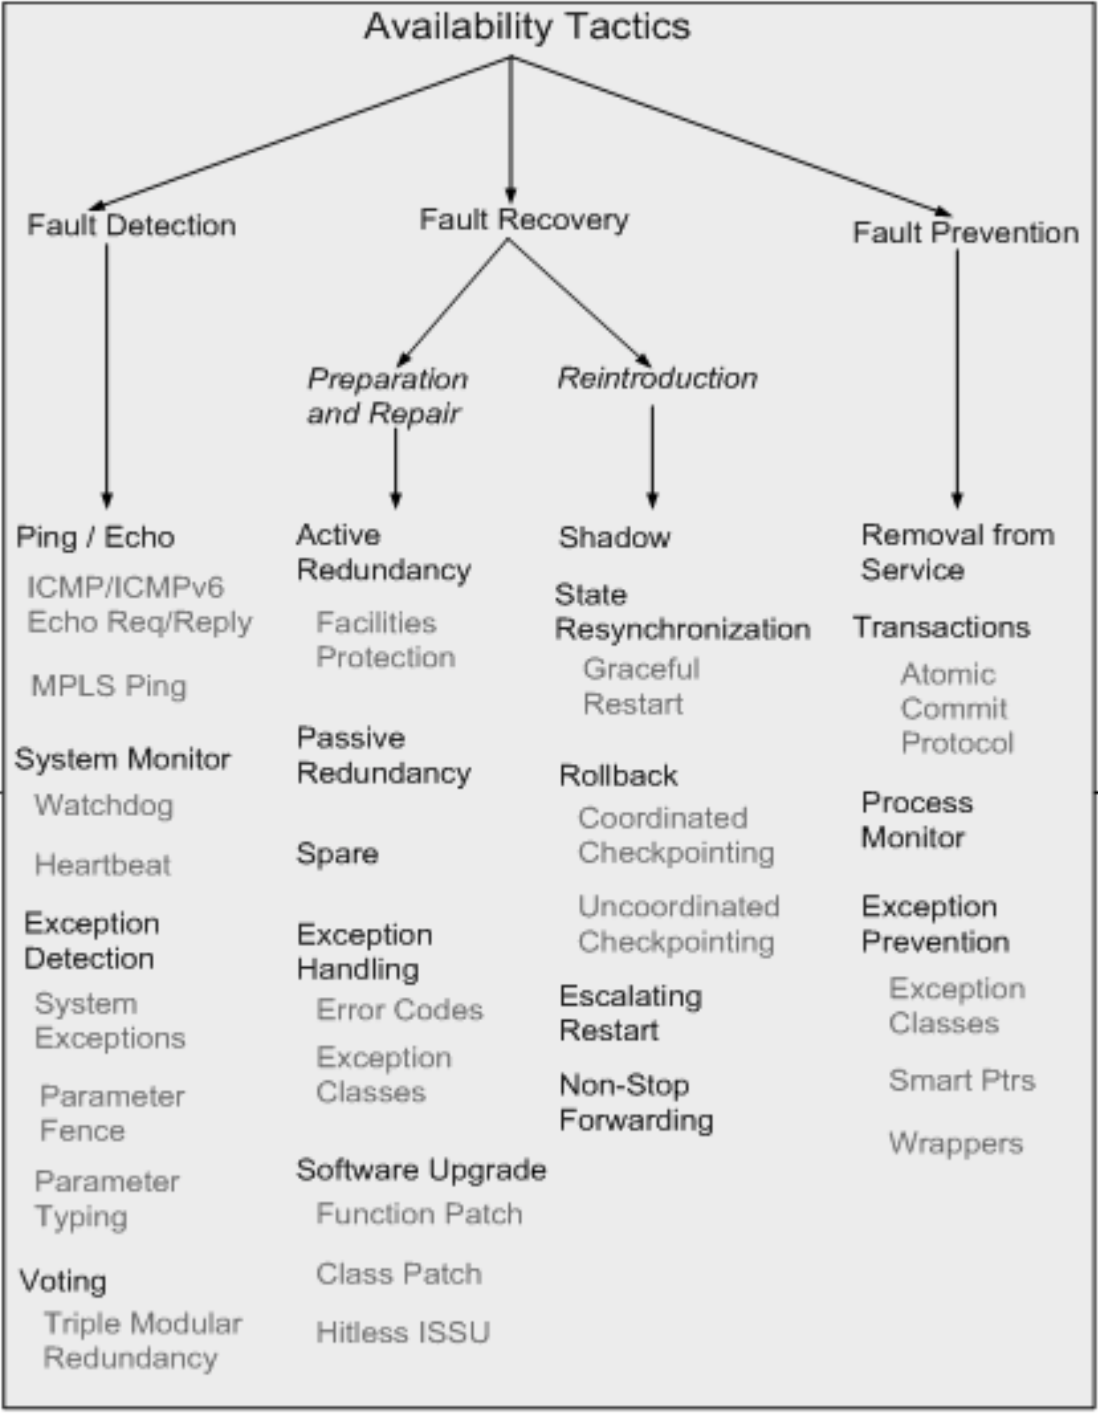
\includegraphics[scale=0.6]{abcdefg.png}
\end{center}

\section{WatchDog}

A watchdog timer (sometimes called a computer operating properly or COP timer, or simply a watchdog) is an electronic timer that is used to detect and recover from computer malfunctions. During normal operation, the computer regularly resets the watchdog timer to prevent it from elapsing, or "timing out". If, due to a hardware fault or program error, the computer fails to reset the watchdog, the timer will elapse and generate a timeout signal. The timeout signal is used to initiate corrective action or actions. The corrective actions typically include placing the computer system in a safe state and restoring normal system operation.\newline
\textbf{Use-Cases: } Embedded Systems, Space Probes, or any system wheree humans cannot easily access the equipment or would be unable to react to faults in a timely manner.

\section{Architectural Design Decisions}
\begin{itemize}
\item{Allocation of responsibilities}
\item{Coordination model}
\item{Data Model}
\item{Management of resources}
\item{Mapping among architectural elements}
\item{Binding time decisions}
\item{Choice of technology}
\end{itemize}

\subsection{Allocation of Responsibilities}

\begin{itemize}
\item{Determine what needs to be high availability (maybe not all functions).}
\item{Responsibility for detecting error (and possible cause).}
\item{Responsibility to log errors}
\item{Responsible respond to a detected error}
\item{Manage sources of events}
\item{Decide on mode of operation}
\item{Decide on how to repair faults}
\item{In the previous case, assign a watchdog and allocate its responsibility of responding to error}
\end{itemize}

\subsection{Coordination Model}
\begin{itemize}
\item{Are the error detection capabilities of the coordination model adequate to detect errors?}
\item{Is the coordination model sufficient to ensure communication and coordination between error detection, log and response.?}
\item{Will coordination work in the presence of error, degraded modes?}
\item{If repair involve replacement of elements will the coordination model allow this?}
\item{In our example the wakeup between watchdog and controller might be an addition to the coordination mechanism.}
\end{itemize}

\subsection{Data Model}
\begin{itemize}
\item{How do error conditions affect the data model?}
\item{Does this mean we have to deal with some forms of corrupt data or incomplete operations?}
\item{Perhaps the data model needs to be extended to include new operations to recover from failed earlier operations.}
\item{For example, extending the model with checkpoint and rollback operations may be enough in some situations.}
\end{itemize}

\subsection{Management of Resources}
\begin{itemize}
\item{See what resources are essential to maintain operation in the presence of errors.}
\item{Identify what resources are necessary for meaningful degraded modes.}
\item{Work out if different scheduling changes the demand on critical resources.}
\item{In our example if task 1 is in error because of a bad processor and task 4 is OK but not necessary for some degraded mode it may be best to switch task 1 and 4 and never schedule task 4 again to provide a degraded mode of operation.}
\end{itemize}

\subsection{Mapping among architectural elements}
\begin{itemize}
\item{Determining what resources might be in error or might be affected by errors.}
\item{Checking that remapping of elements is possible dynamically.}
\item{How fast can elements be restarted or reinitiallised, can a process be moved to a new processor, …}
\item{In our example it may be necessary to identify the watchdog as a new element and that a failing task may need to be mapped to a different processor.}
\end{itemize}
\subsection{Binding Time Decisions}
\begin{itemize}
\item{Look at binding time and see where this will allow flexibility.}
\item{For example, if we can tolerate a 0.5s delay on a response but are currently using 0.1s as the time to signal an error then we might want to rebind and operate in a degraded mode.}
\item{In our example, if the the taks code is burned into PROMS on the processors there is no chance to rebind task/processor.}
\end{itemize}
\subsection{Choice of Technology}
\begin{itemize}
\item{Explore technologies that package useful functionality for availability.}
\item{Use an established element if it is available.}
\item{Use already established data on the availability characteristics of components.}
\end{itemize}

\chapter{7. Performance}

\section{Performance General Scenario}
\begin{tabular}{||c | c||} 
 \hline
 Portion Of Scenario & Possible Values \\ [0.5ex] 
 \hline\hline
 No Dropout, Baseline &  \\ 
 \hline
 Source & Internal or External to the System \\
 \hline
 Stimulus & Arrival of a periodic, sporadic or a stochastic event \\
 \hline
 Artifact & System or one or more components in the system \\
 \hline
 Environment & Operational Mode: Normal, Emergency, Peak, Overload  \\
 \hline
 Response & Process Events, Changed level of service \\ 
 \hline
 Response Measure & Latency, deadline, throughput, jitter, miss rate \\
 \hline
\end{tabular}
\newline
\newline
A Typical Scenario:
\begin{center}
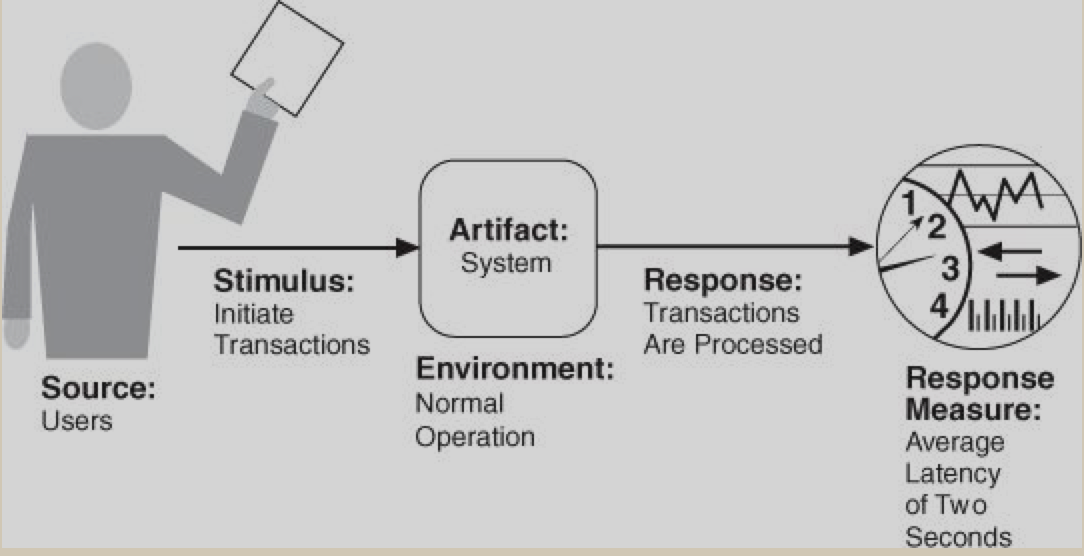
\includegraphics[scale=0.6]{sad.png}
\end{center}

\section{Making the Scenario Specific}
We need to say something about the distribution of the arrival of the stimuli.
\begin{itemize}
\item{E.g. The inter-arrival time is always greater than 1.0 secs}
\item{How is this different from the arrival rate is less than 1 per second?}
Any stimulus needs to be processed within 2 seconds of arriving.
The responses should appear in the same order as the stimuli.
\end{itemize}

\section{A Possible Architecture}

Queue $\rightarrow$ Process $\rightarrow$ Output

\section{Being Specific About the Architecture}

We need to say something about the capacity of the processor:
\begin{itemize}
\item{The worst case processing time for a stimulus is 1.5 seconds best case time is 1.0 secs}
\item{The processor can only process one stimulus at a time.}
We need to say that the queue capacity is 7 stimuli (or some other).
This architecture fails the scenario (why?)
\end{itemize}

\section{Performance Tactics}
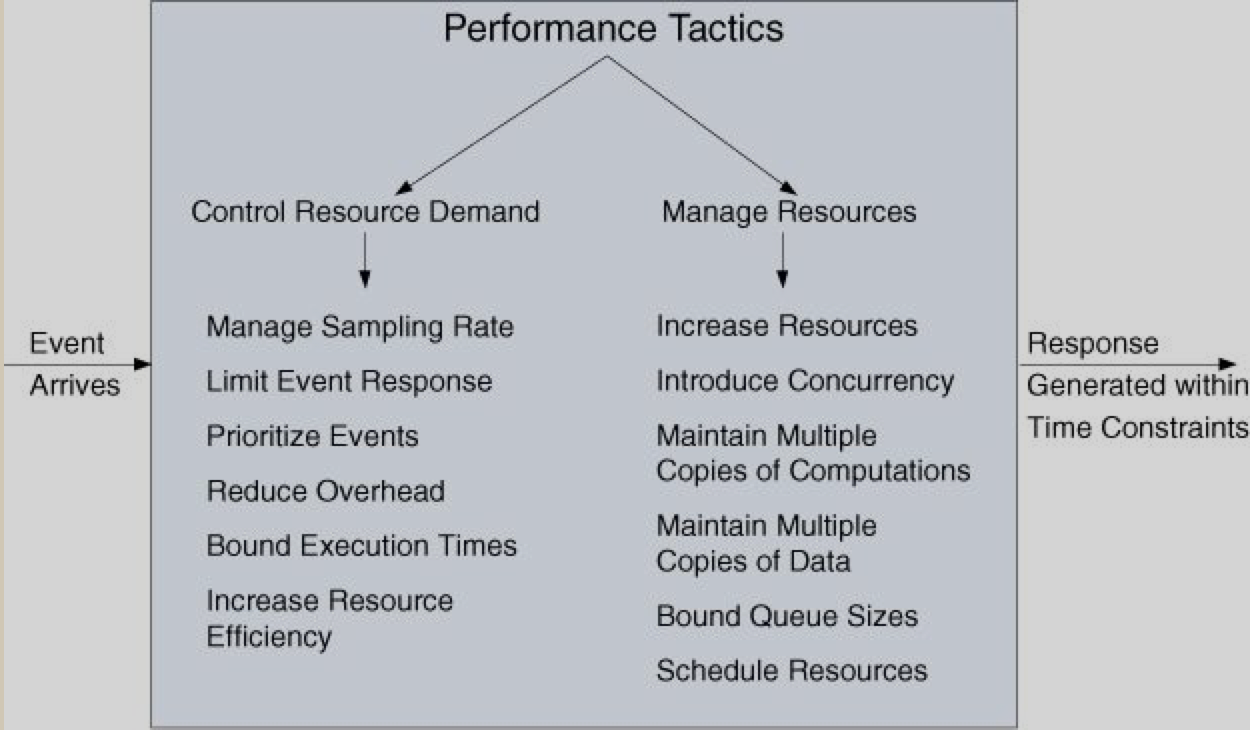
\includegraphics[scale=0.6]{zxc.png}

\section{Control Resource Demand Tactics}

\begin{itemize}
\item{\textbf{Manage the sampling rate} (not always applicable) – ensure you do not have too much to handle.}
\item{\textbf{Limit the event response} – if you are receiving too many events, throw some away.}
\item{\textbf{Prioritize events} – some need a respons in a certain time – some don’t}
\item{\textbf{Reduce overhead} – can you take resource out of handling an event?}
\item{\textbf{Improve the efficiency of processing} – so you can handle more with the same processing}
\end{itemize}

\section{Manage Resources}

\begin{itemize}
\item{Increase resources}
\item{Introduce concurrency}
\item{Maintain multiple copies of compute and/or data}
\item{Bound queue sizes}
\item{Schedule resource when there is contention (hard scheduling for highest priority events)}
\end{itemize}

\section{Checklist: Allocation of Responsibilities}
\begin{itemize}
\item{Work out areas responsibility of that require heavy resource use to ensure time-critical events take place.}
\item{Work out processing requirements.}
\item{Take account of:
	\begin{itemize}
	\item{Responsibilites arising from threads crossing boundaries of responsibility}
	\item{Responsibilities for thread management}
	\item{Responsibilities for scheduling shared resources}
	\end{itemize}
}
\end{itemize}

\section{Checklist: Coordination Model }
\begin{itemize}
\item{What needs to coordinate.}
\item{Is there concurrency?  Ensure it is safe.}
\item{Ensure coordination is appropriate for the style of stimulus.}
\item{Ensure the properties of the coordination model are good for the stimuli and concurrency control?}
\end{itemize}

\section{Checklist: Data Model}
\begin{itemize}
\item{Determine what parts of the data model will be heavily loaded or have tight time constraints.}
\item{Then:
\begin{itemize}
\item{Would keeping multiple copies help?}
\item{Would partitioning the data help?}
\item{Is it possible to reduce processing requirements for the data?}
\item{Does adding resource help deal with data bottlenecks?}
\end{itemize}}
\end{itemize}

\section{Checklist: Mapping Among Architecture Elements }
\begin{itemize}
\item{Does colocation of some components reduce latencies?}
\item{Ensure components with high processing needs are allocated to big processors}
\item{Consider introducing concurrency when you map.}
\item{Consider whether some mappings introduce bottlenecks (e.g. allocating non-interfering tasks to the same thread)}
\end{itemize}

\section{Checklist: Resource Management}
\begin{itemize}
\item{Work out what needs high levels of resource}
\item{Ensure these are monitoredand managed under all operating modes.}
\item{For example:
\begin{itemize}
\item{Time critical components}
\item{Thread management}
\item{Prioritization}
\item{Locking and scheduling strategies}
\item{Deploying additional resource to meet elevated load.}
\end{itemize}
}
\end{itemize}


\section{Checklist: Binding Time}
\begin{itemize}
\item{Look at when you bind.}
\item{Consider the cost of binding at different times.}
\item{Try to avoid performance penalties caused by late binding.}
\end{itemize}

\section{Checklist: Choice of Technology}
\begin{itemize}
\item{Is the technology right to let you meet hard deadlines and resource use (e.g. use a real-time OS with proper scheduling).}
\item{You need:
\begin{itemize}
\item{Good scheduling}
\item{Priorities}
\item{Policies for demand reduction}
\item{Allocating processing to tasks}
\item{Other performance-related measurement and management.}
\end{itemize}}
\end{itemize}













\end{document}
